\chapter{Coding}
\label{chapter:coding}

some text here....

c++
opencv
wxwidgets
libcamera


\section{View Implementation}
As discussed previously in Chapter \ref{sec:model-view-controller}, the view is responsible for displaying the data to the user, in other words,  it defines the user interface and displays the information from the model \cite{Krastev20}. In this section, the implementation of the view is discussed in detail.

To further streamline the development process of view, we have set up a set of guidelines that we have followed throughout the development process. These guidelines are as follows:

\subsubsection{Handling User Input}
This guideline emphasizes that the View should be adept at managing and processing user interactions. It is responsible for capturing user inputs, such as mouse clicks, keyboard entries, or touch gestures, and conveying them to the Controller for further processing. This can involve events like form submissions, button clicks, or interactions with interactive elements on the user interface.

\subsubsection{Avoid any business logic}
This directive underscores the importance of maintaining a clear separation of concerns within the MVC architecture. The View should refrain from incorporating any form of business logic, which involves tasks like data validation, computation, or decision-making processes. Instead, these responsibilities are delegated to the Model and Controller components. By adhering to this guideline, the View remains focused on its core function of presenting data and interacting with the user interface.

\subsubsection{Avoiding Direct Model Manipulation}
This guideline reinforces the principle of ensuring that the View does not directly modify the state or data of the Model. Instead, any alterations to the underlying data should be orchestrated through the Controller. This establishes a controlled flow of data within the application, maintaining data integrity and adherence to the MVC architectural pattern.

\subsubsection{Utilizing Templates or Layouts}
This recommendation advocates for the adoption of templating engines or layout systems in view development. These tools facilitate the creation of modular, reusable components that can be dynamically combined to construct the user interface. By employing templates or layouts, developers streamline the process of designing and rendering the View, resulting in a more maintainable and scalable codebase.

\subsubsection{Error Handling and Feedback Mechanisms}
This guideline emphasizes the necessity of implementing robust error handling mechanisms within the View. It is imperative to provide clear and informative feedback to the user in the event of errors or invalid inputs. This ensures that users are guided through the application's workflow, even in scenarios where unexpected events occur. Effective error handling contributes to a more user-friendly and reliable user experience.

\subsection {Main Layout}
The implementation of the main layout is the first step in the development of the view. The main layout is the universal layout that is used throughout the application. The implementation is done based on the result of the wireframing process which is done in Section \ref{subsec:wireframe}.

\begin{figure}[!ht]
    \centering
    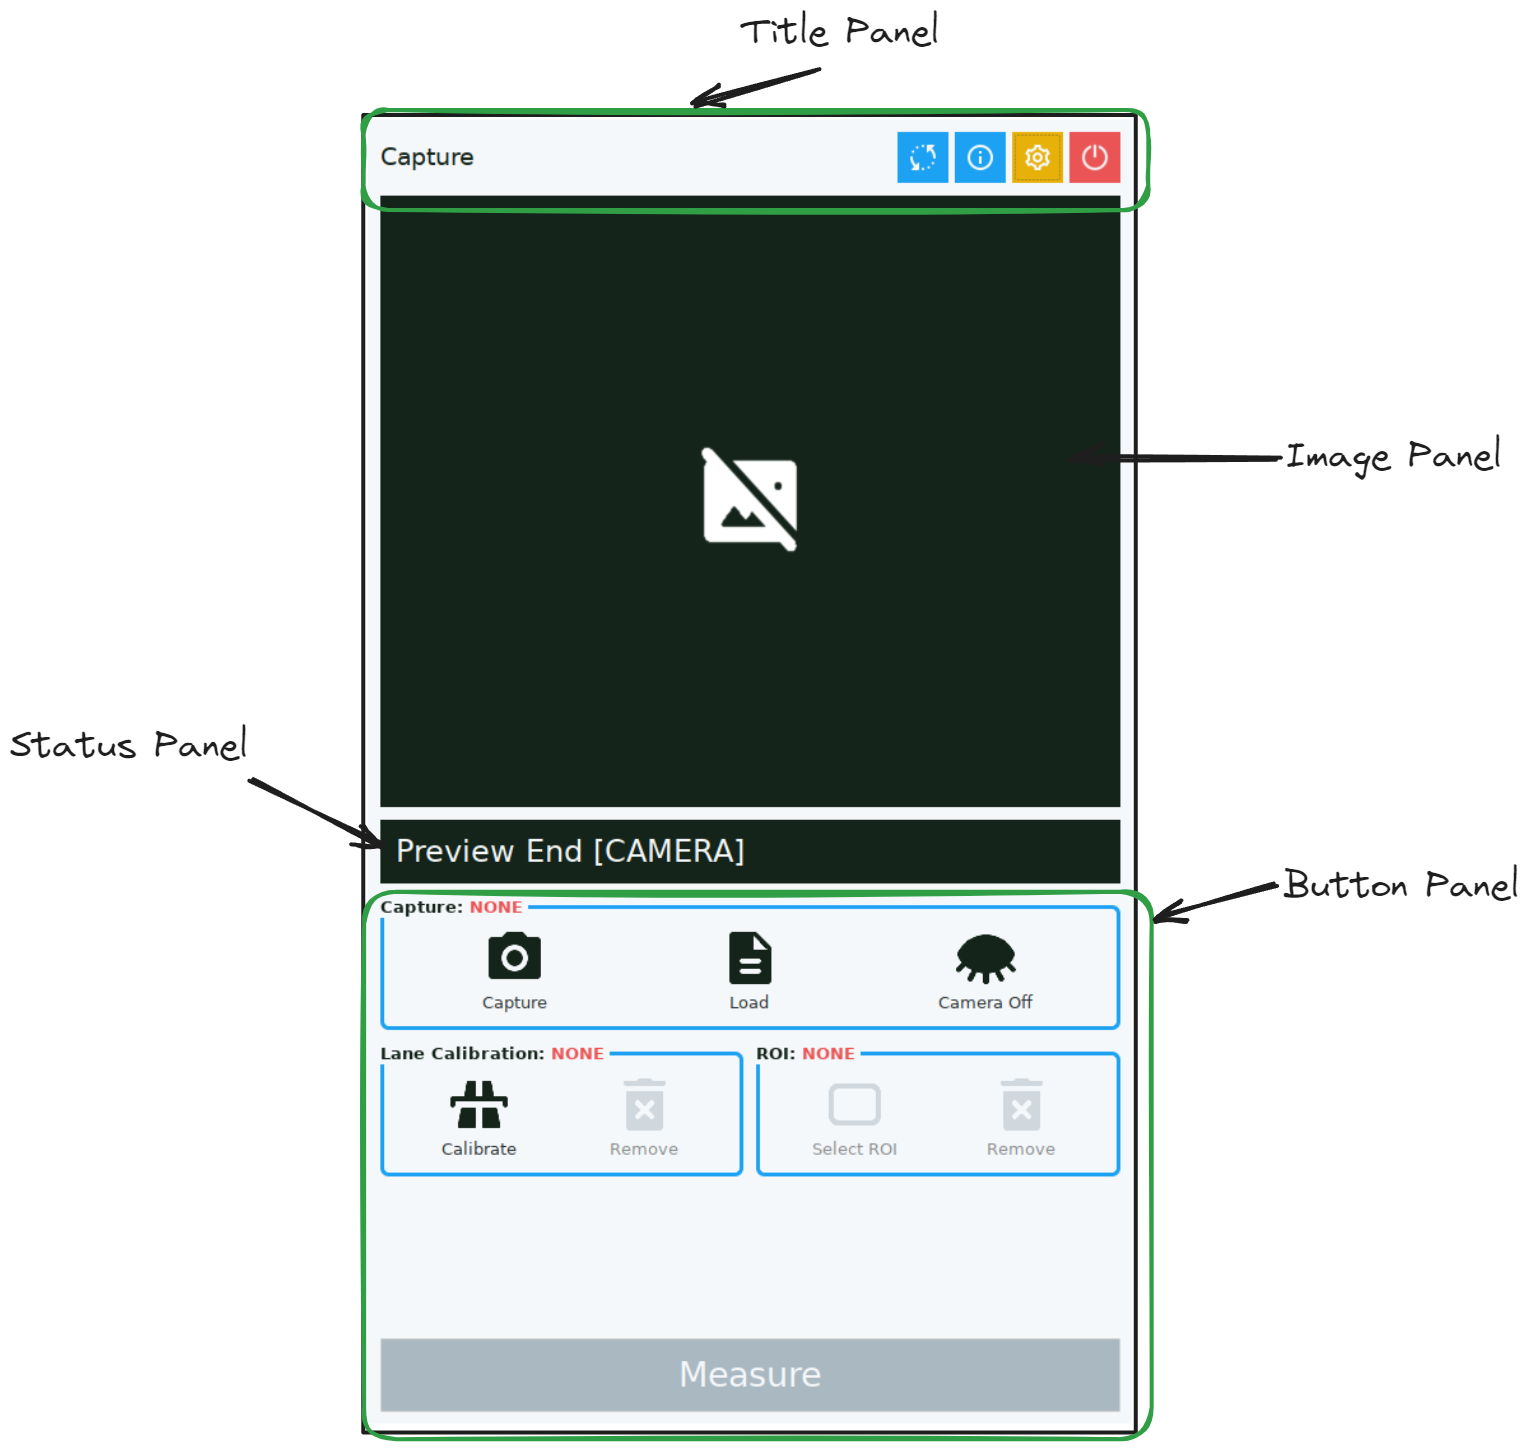
\includegraphics[width=0.45\textwidth]{texs/Part2/chapter4/image/mainlayout.png}
    \caption{Main Layout}
    \label{fig:main_layout}
\end{figure}

The main layout is shown in Figure \ref{fig:main_layout}. The main layout consists of a title panel, image panel, status panel and button panel. All of the function of the components are explained previously in Section \ref{subsec:wireframe}.



\subsection{Bitmap Button}
Bitmap Button is a type of button that is mainly used within the application. It contain a bitmap image and a text lable positioned on below the image. Figure \ref{fig:bitmap_button} shows a couple of bitmap buttons that are used within the application.

\begin{figure}[!ht]
    \centering
    
\includegraphics[width=0.45\textwidth]{texs/Part2/chapter4/image/bitmapbutton.png}
    \caption{Bitmap Button}
    \label{fig:bitmap_button}
\end{figure}

Throughout the implementation process, there are 3 different types of
bitmap button implemented. They are Type 1, Type 2 and Type 3. Two of these types, Type 1 and Type 2, share a similar design concept, but it differ in its state handling.

Figure \ref{fig:type1_state} shows  the button appearance on different states. This type of buttons are useful when the button is used to trigger a process that require a long time to complete.  For example, in the context of capturing an image, the button assumes a 'normal' state when no image has been captured. When pressed, the process commences, and the button transitions to an 'active' state, signifying that the process is underway. During this active state, the button is also 'disabled' to prevent any potential interruptions or inadvertent re-triggering of the process. Once the process is successfully completed, the button shifts to a 'disabled' state, indicating that the process cannot be re-initiated.

\begin{figure}[!ht]
    \centering
    
\includegraphics[width=0.45\textwidth]{texs/Part2/chapter4/image/type1state.png}
    \caption{Type 1 Button State}
    \label{fig:type1_state}
\end{figure}

\begin{figure}[!ht]
    \centering
    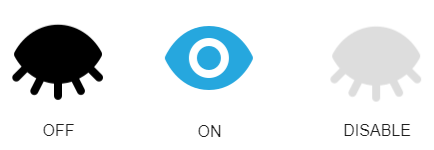
\includegraphics[width=0.45\textwidth]{texs/Part2/chapter4/image/type2state.png}
    \caption{Type 2 Button State}
    \label{fig:type2_state}
\end{figure}


The states for Type 2 button are shown in Figure \ref{fig:type2_state}. This type of button is used when the button is used to trigger a process that require toggeling. For instance, in the context of turning on a camera, the button assumes an 'off' state when the process has not been initiated and is available for activation. Upon pressing the button, the process initiates, and the button transitions to an 'on' state, indicating that the process is actively running. If necessary, pressing the button again will revert the state back to 'off', effectively terminating the ongoing process.

\begin{figure}[!ht]
    \centering
    
\includegraphics[width=0.45\textwidth]{texs/Part2/chapter4/image/type3state.png}
    \caption{Example of Type 3 Button}
    \label{fig:type3_state}
\end{figure}

The last type of bitmap buttons is Type 3. In terms of appearance, it differs from the previous two types. This button contains only bitmap image, without the text label, and coloured backgrounds. It does not have states, and it is used to trigger a  very simple straightforward process, such as exiting the application or opening the settings panel.
This type of buttons can be seen in the title panel (see Figure \ref{fig:type3_state}).

\subsubsection{Handling Button Input}
\label{subsubsec:handling_button_input}
The process of handling button input is done by using event handling mechanism provided by wxWidgets. For a more detailed explanation on how the event handling mechanism works, please refer to wxWidgets Documentation \cite{wxWidgetsEvent}.

In general, the process of handling button input is done by binding the button to a function. By pressing the button, an event is triggered, and the function is executed. Depending on the implementation, different button can trigger different function. For example, the button to turn on the camera will trigger a function to turn on the camera, while the button to capture an image will trigger a function to capture an image.

This process can be dony by assigning a unique ID to each button. By doing so the button can be identified and binded to a specific function. Following is a short example of how the button is binded to a function.

\subsubsection{Updating Button State}
A proper feedback mechanism is essential to ensure that the user is aware of the current state of the application. In the context of the application, the button state is used to provide feedback to the user on the current state of the application. For example, when the user interact with a button to turn on camera, the feedback to the user is the button state changes from 'off' to 'on'.

The process of updating button state is done by using event handling similar to the process of handling button input. Whenever an update is required, for example, after a button pressed, or after a process is completed, an event is triggered, and the button state is updated accordingly. This process is usually done by the controller component, as it is responsible for handling the application logic.

However it is also important to note that while updating component state is crucial, updating it too frequently can be detrimental to the application performance. Therefore, it is important to find a balance between the two.

\subsection{Error Handling and Feedback Mechanisms}
\label{subsec:error_handling_and_feedback_mechanisms}
In real world scenarios, errors are inevitable. Therefore, it is important to implement a proper error handling mechanism to ensure that the user is guided through the application's workflow, even in scenarios where unexpected events occur. Effective error handling contributes to a more user-friendly and reliable user experience.

In the context of the application, the error handling mechanism is implemented by using a message dialog. A message dialog is a dialog that displays a message to the user, along with buttons for the user to click.Figure \ref{fig:message_dialog} shows an example of a message dialog.

The \textit{ErrorEvent} can be utilized to display an error message to the user. When an exception is thrown during a process, an \textit{ErrorEvent} will be created by the controller component and passed to the view component. The view component will then display the error message to the user by using a message dialog.


\subsection{Image Panel}
\label{subsec:image_panel}

\subsubsection{Displaying Image to the User}
The image panel is the component that is responsible for displaying the image to the user. To display image to the user, the \textit{UpdatePreviewEvent} is used. For example, when turning on the camera, a thread controller will initialized a thread which responsible for the process of capturing image from camera. For each iteration, the thread will capture an image and create the \textit{UpdatePreviewEvent} and pass it to the view component. The image panel will catch the event and display the image to the user.

\subsubsection{Handling Touch Input}
\label{subsubsec:handling_touch_input}
touch input can be  used ad another method of user input. The process of handling touch input is similar to the process of handling button input. It can be done by binding the touch event to a function. By doing so, whenever a touch event is triggered, the function will be executed.

The implementation via event by wxwidgets such as wxMouseEvent. Alternatively, the implementation can also be done by utilizing the \textit{BasePanelWithTouch} class when implementing the views. This class already contains the implementation of touch event handling, and  methods to handle the events are also included. For more information, please refer to project Documentation on \ref{appendix:documentation}.

\subsection{Navigating between different panel}
\label{subsec:navigating_between_different_panel}

For this application, multiple panels or views are implemented based on its functionality. For example, the capture panel is used to capture an image, while the calibration panel is used to perform camera calibration. Since multiple views are implemented, a proper method in displaying the views to the user is required.

Therefore to simplify the process, we have set that within the frame, only one view can be displayed, while others are kept hidden. This is done by using the \textit{Show()} and \textit{Hide()} method provided by wxWidgets. When navigating to a different view, the current view will be hidden, and the new view will be shown.

Figure \ref{fig:show_panel} shows an example of navigating between different panel by using \textit{Show()} and \textit{Hide()} method.

\begin{figure}[!ht]
    \centering
    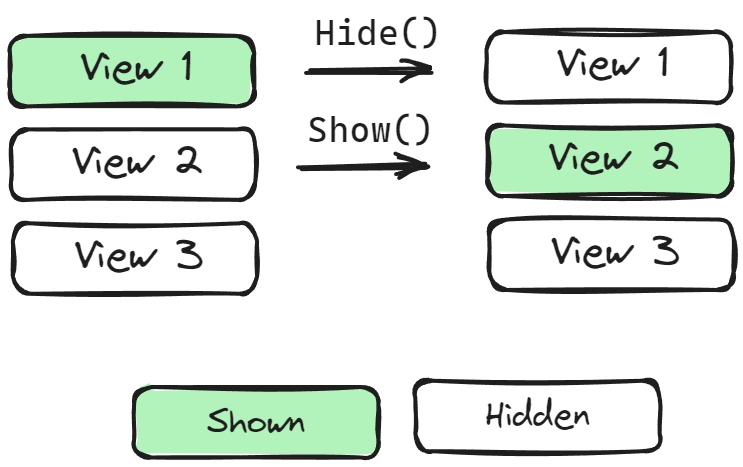
\includegraphics[width=0.45\textwidth]{texs/Part2/chapter4/image/showpanel.png}
    \caption{Example of navigating between different panel}
    \label{fig:show_panel}
\end{figure}

\section{Model Implementation}
\label{sec:model_implementation}

\subsection{Model Overview}
\label{subsec:model_overview}
In this section, the overview of the model is provided. The model is responsible for storing the data and the application logic. Figure \ref{fig:model_overview} shows the overview of the model.

\begin{figure}[!ht]
    \centering
    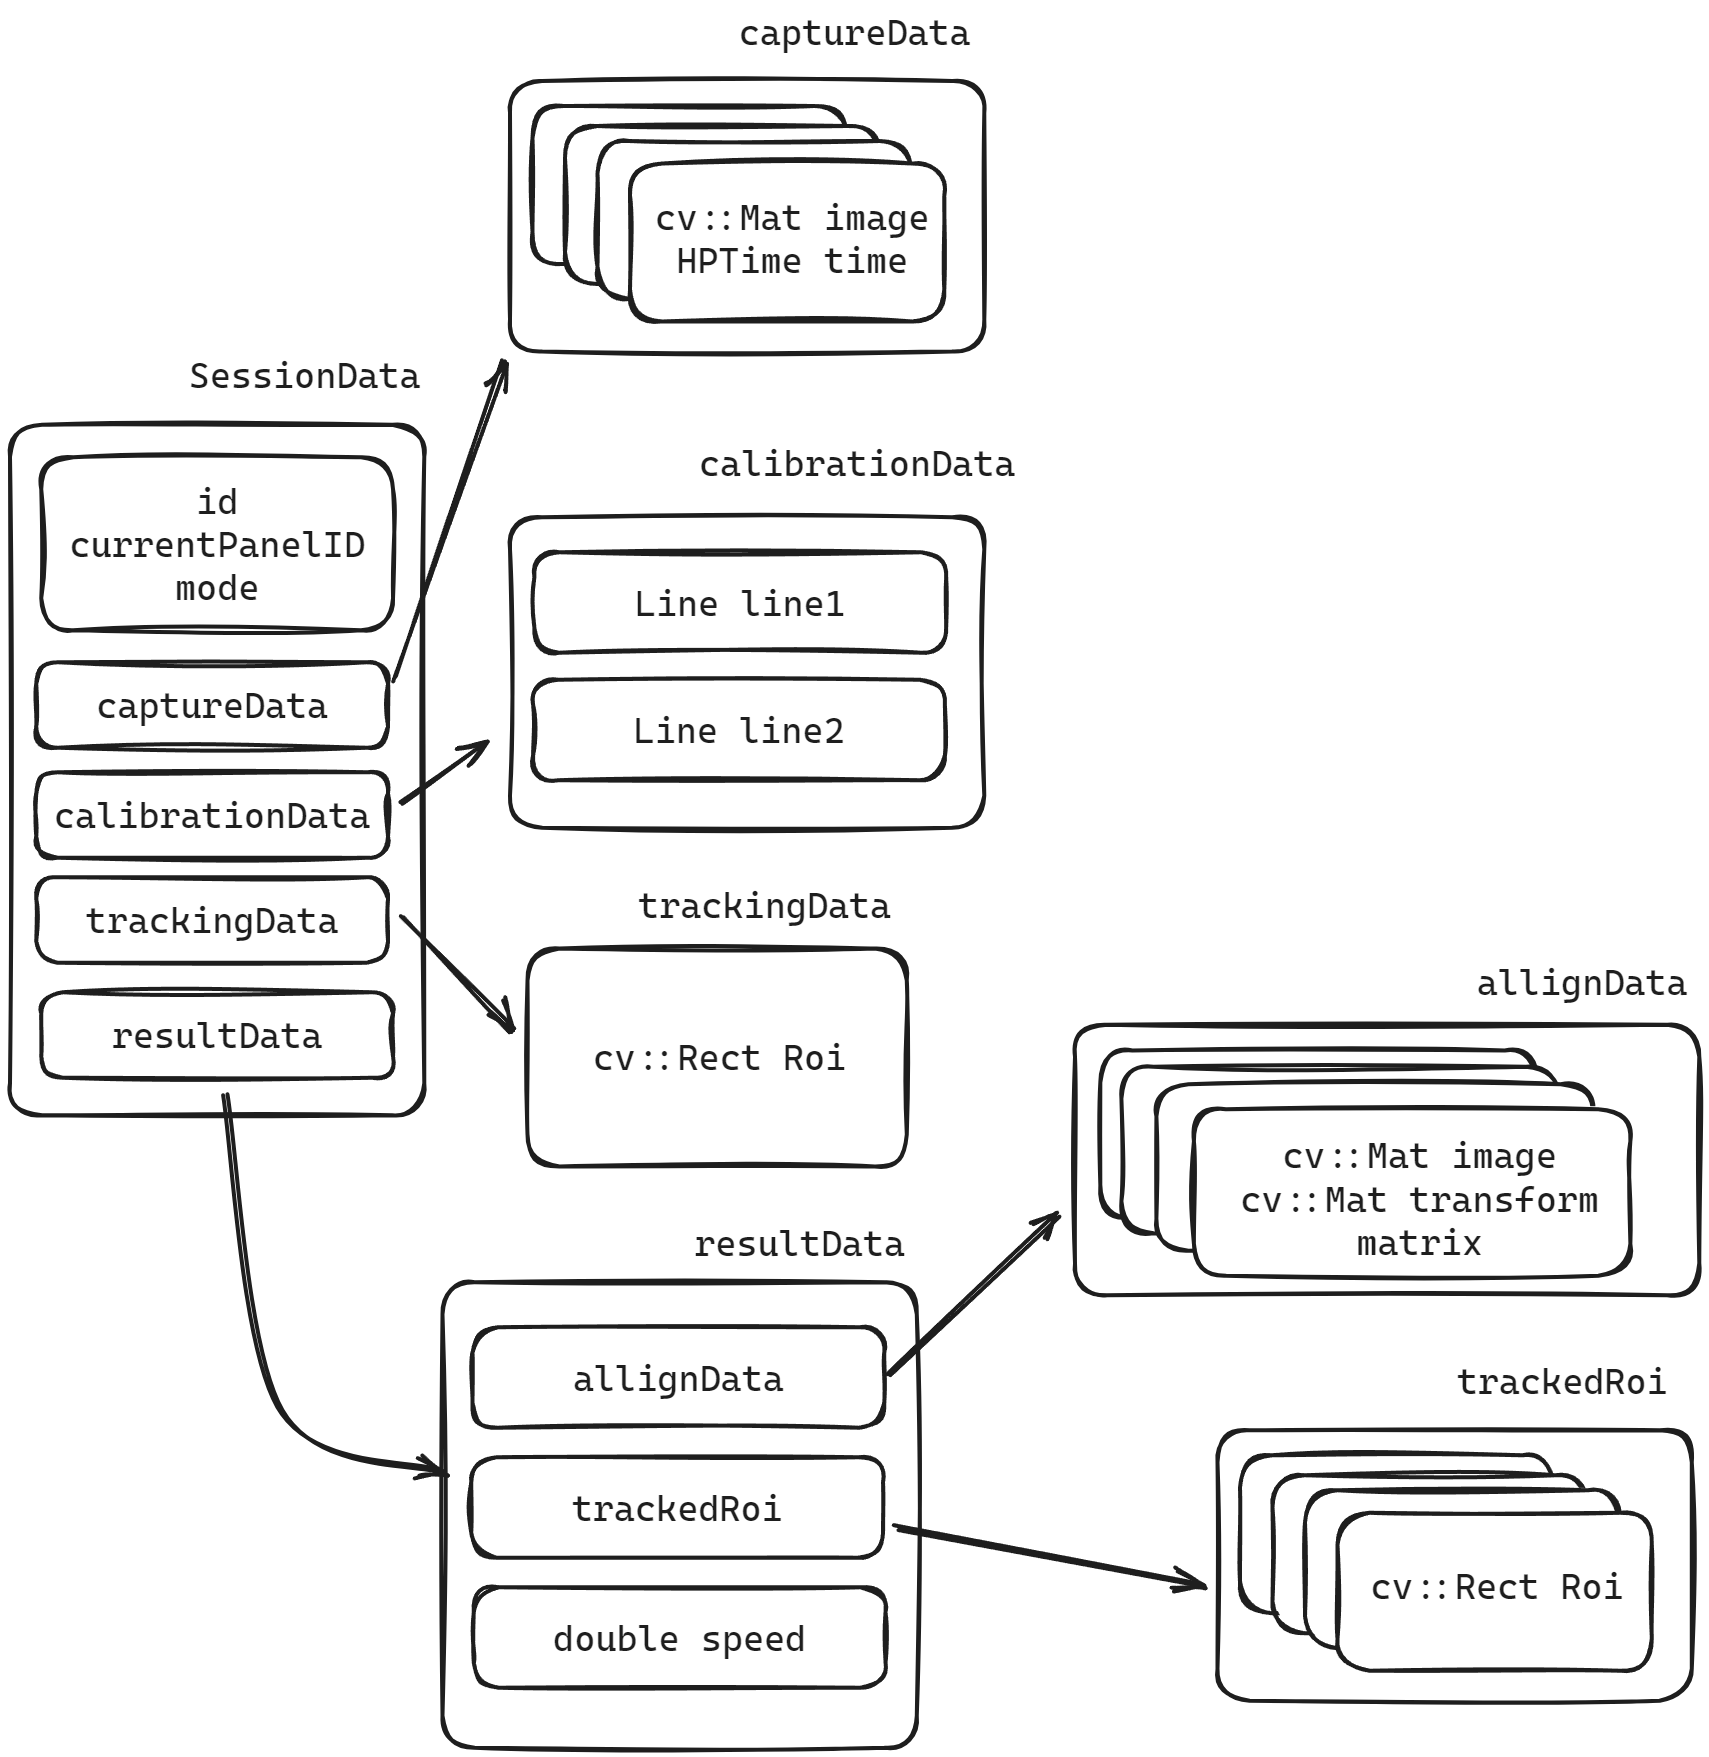
\includegraphics[width=0.75\textwidth]{texs/Part2/chapter4/image/sessiondata.png}
    \caption{Overview of Model}
    \label{fig:model_overview}
\end{figure}

The model consists of 5 main components, which are \textit{SessionData}, \textit{captureData}, \textit{calibrationData}, \textit{trackingData} and \textit{resultData}. Each of these components is explained in detail in the following sections.

\textbf{SessionData:} Responsible for storing the current overall state of the application. The \textit{id} variable describe the current id of the session, while \textit{currentPanelID} provide information on current active panel to be rendered by the application. \textit{Mode} describe on which calculation mode is choosen by the user. For more information on \textit{mode}, please refer Section \ref{}.

\textbf{CaptureData:} This data stores a vector of original images captured by the camera. Alongside the image, this data type also responsible to store the time on which the image is captured, to be used for measurement purpose.

\textbf{CalibrationData:} Contains the result of calibration process, which are the variables \textit{line1} and \textit{line2}. For more information on these variables, please refer to Section \ref{subsec:calibration_process}.

\textbf{TrackingData:} This data stores the initial region of interest (ROI) on which the tracked object is located.

\textbf{ResultData:} This data stores the result of the calculation process. Within this data, there are 3 variables, which are \textit{allignData}, \textit{trackedRoi} and \textit{speed}. \textit{allignData} stores the result of the allignment process, while \textit{trackedRoi} stores the result of the tracking process. \textit{Speed} variable is the value of the speed of the tracked object, which is calculated by using the result of the allignment process and the result of the tracking process.

\section{Controller Implementation}
\label{sec:controller_implementation}

\subsection{Individual Controller}
\label{subsec:individual_controller}

As mentioned previously in Section \ref{}, each view will have its own controller associated to it. By doing so, each controller will each have its own responsibility, which is to handle the application logic for the view. Furthermore, this design also helps in terms of application scaling. By having multiple controllers, the application logic can be divided into smaller parts, which makes it easier to maintain and scale.

However, a proper controller design guidelines are required to ensure that these controllers are implemented properly. Therefore, we have set up a set of guidelines that we have followed throughout the development process. These guidelines are as follows:

\subsubsection{Only handle request and response}
This guideline emphasizes that the controller should only handle request and response. It should not contain any business logic. Instead, the business logic should be implemented in the threads, which will be discussed in Section \ref{subsec:thread_and_thread_controller}.

\subsubsection{Provide similar endpoints}
To ensure proper communication between the controller and the view, it is important to provide similar endpoints for each controller. By doing so, developers can easily identify the methods that are responsible to communcate between the views and the controller. To properly implement this guideline, all methods which are responsible for communication between the view and the controller should be named with the prefix \textit{e\_}, which stands for \textit{endpoint}. For example \textit{e\_startCamera()}, \textit{e\_captureImage()} and \textit{e\_calibrate()}.

\subsubsection{Only handle one view}
This guideline emphasizes that the controller should only handle one view. This is to ensure that the controller is not overloaded with too many responsibilities. By doing so, the controller can be easily maintained and scaled.

\subsubsection{Singular responsibility}
Each endpoint should only handle one responsibility. For example \textit{e\_startCamera()} should only handle the process of starting the camera, and not other process such as capturing an image or calibrating the camera.

\subsubsection{Handle error}
All endpoints should be wrapped with a try-catch block to handle any error that might occur during the process. If an error occurs, an \textit{ErrorEvent} will be created and passed to the view component. The view component will then display the error message to the user by using a message dialog. For more information on how the error handling mechanism works, please refer to Section \ref{subsec:error_handling_and_feedback_mechanisms}.

\subsubsection{Prevent handling outside active panel}
\label{subsec:prevent_handling_outside_active_panel}
This guideline emphasizes that the controller should only handle request and response when the view is active. This strict rule is implemented to prevent any unwanted behaviour that might occur when the view is not active. The \textit{checkPrecondition()} provide method to check whether the view is active or not. If the view is not active, error message will be displayed to the user.

\subsection{Threads and Thread Controller}
\label{subsec:thread_and_thread_controller}
To reduce the responsibility of the controller, the process of handling the business logic is delegated to the \textit{threads}. By seperating the execution of business logic on different threads, it prevents the main thread or the GUI thread from being blocked. This is important to ensure that the application is responsive and does not freeze.

Additionally the threads also has the access to the thread pool, to take leverage of parallel execution whenever required. The \textit{thread controller} is responsible to manage the threads by starting, stopping and joining the threads. Furthermore the thread controller also responsible to provide status on the current state of the threads, either it is running or not.

Table \ref{table:thread_controller} shows the list of threads that are implemented within the application.

% \begin{table}[!ht]
%     \centering
%     \begin{tabularx}{\textwidth}{|X|X|}
%         \hline
%         \textbf{Event}         & \textbf{Purpose}                      \\ \hline
%         CalibrationEvent        & Signal status of calibration process  \\ \hline
%         ChangePanelEvent        & Handle changing panel                 \\ \hline
%         ErrorEvent              & Error Handling                        \\ \hline
%         LoadImageEvent          & Use in capturing or load image data   \\ \hline
%         PreviewEvent            & Display current calibration data      \\ \hline
%         ProcessImageEvent       & Signal status of processing image     \\ \hline
%         ReplayEvent             & Signal status of replay thread        \\ \hline
%         RequestUpdateStateEvent & Request view to update state          \\ \hline
%         RoiEvent                & Signal status of ROI selection thread \\ \hline
%         SaveDataEvent           & Saving data to binary                 \\ \hline
%         UpdatePreviewEvent      & Update image panel with new image     \\ \hline
%         UpdateStateEvent        & Update state                          \\ \hline
%         UpdateStatusEvent       & Update status panel                   \\ \hline
%     \end{tabularx}
%     \caption{List of Implemented Threads}
%     \label{table:thread_controller}
% \end{table}

\subsection{Request Handling Example}
\label{subsec:request_handling_example}

In this section, an example of how the request is handled by the controller is provided. A sequence diagram is used to illustrate the process, as shown in Figure \ref{fig:sequence_diagram}.

\begin{figure}[!ht]
    \centering
    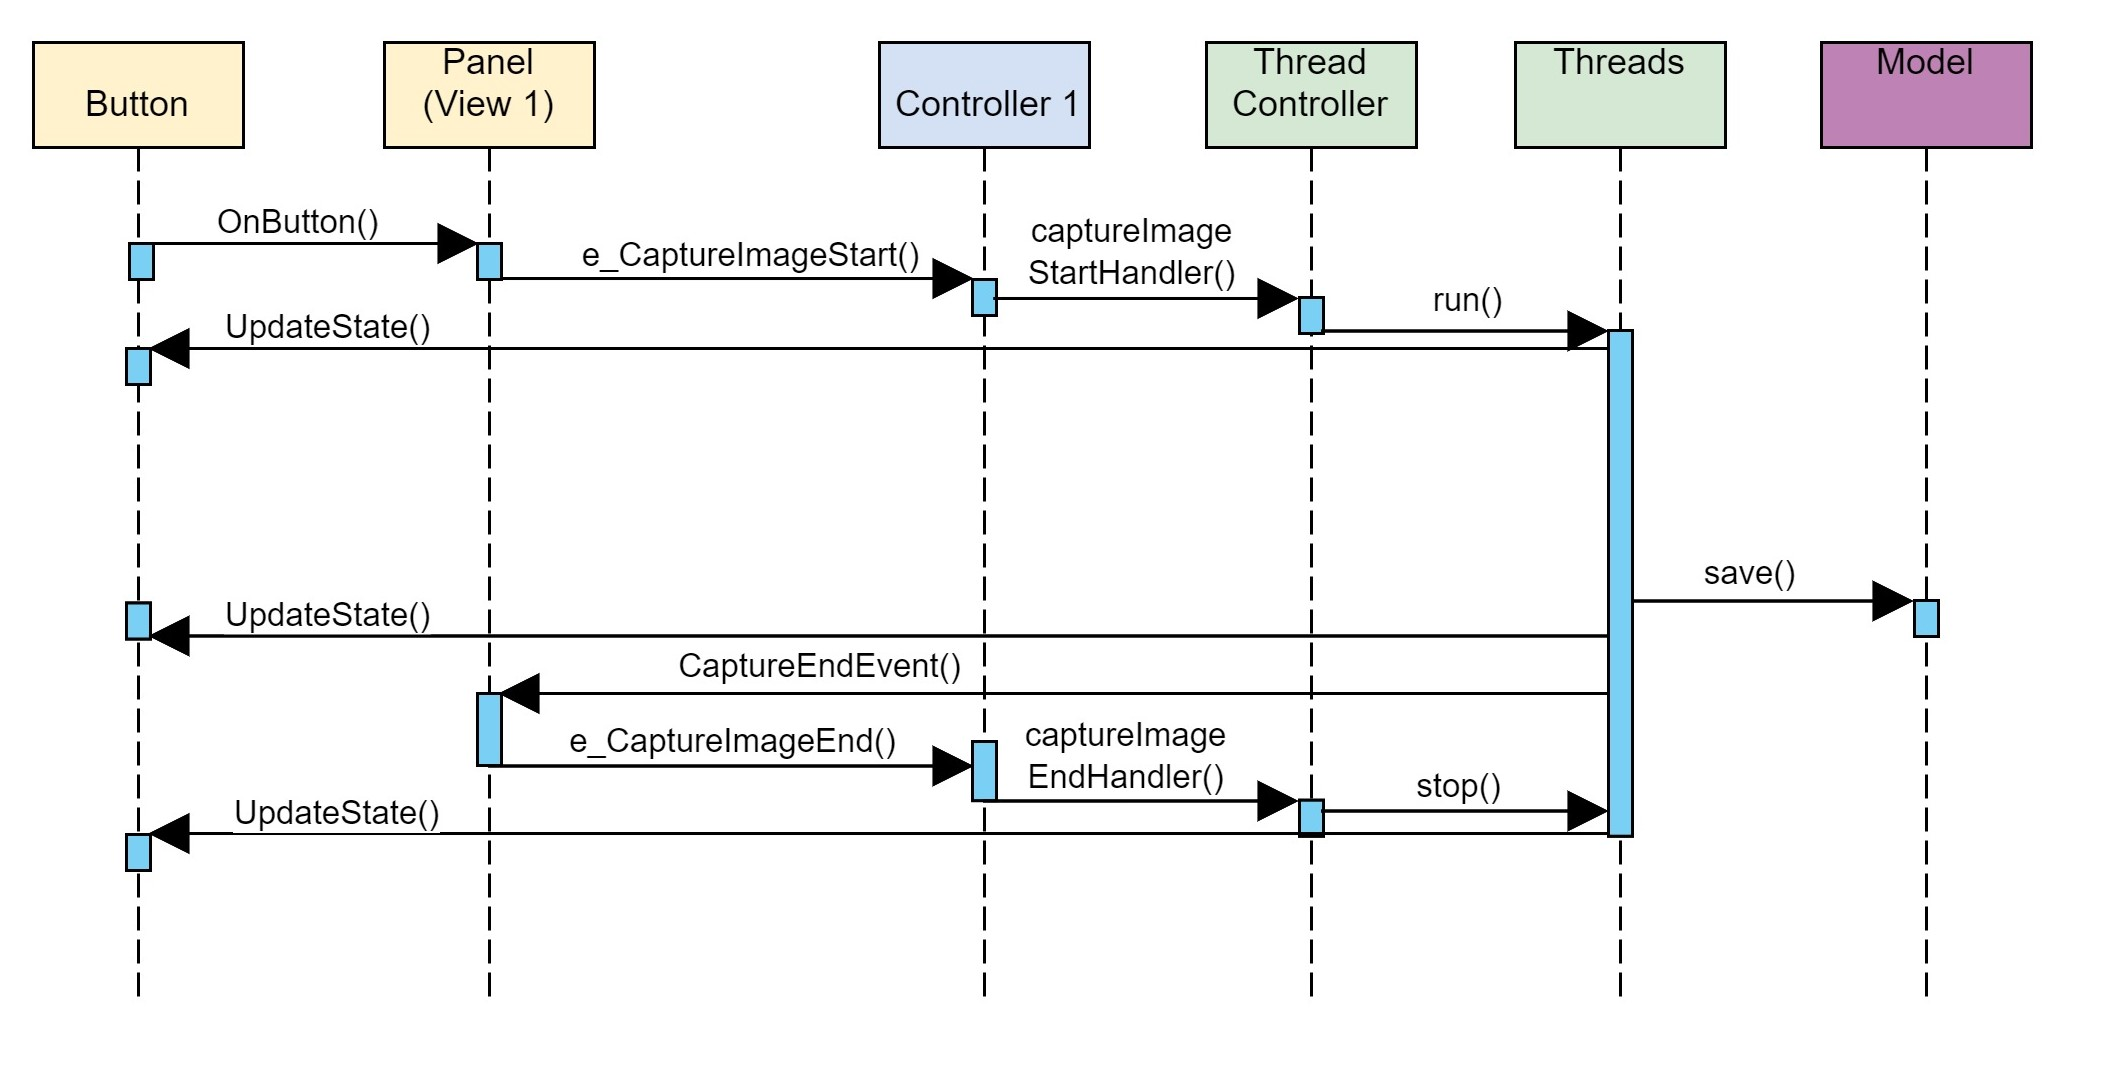
\includegraphics[width=0.9\textwidth]{texs/Part2/chapter4/image/sequence.jpg}
    \caption{Example of Request Handling}
    \label{fig:sequence_diagram}
\end{figure}

With this example, the request starts by pressing a button. This action will trigger an event, which will be handled by the \textit{View1}. The view will then request for an initialization of process or thread via the endpoint \textit{e\_CaptureImageStart()}. The request will be forwarded to the \textit{ThreadController} and a threads to capture image is spawned. The state is updated to signal the succession of the request. The thread will run on its own, and when it finished capturing image, the data is saved to the model via the \textit{save()} method. The state is once again updated and an event signaling the completion of the process is sent to the view. With this event, the view signal the controller to stop the thread via the endpoint \textit{e\_CaptureImageStop()}. The thread is then stopped and joined. The state is updated to signal the completion of the process.

\section{Algorithm Improvement}
\label{sec:algorithm_improvement}

\subsection{Image Alignment}
Based on previous work \cite{Sabtu_2023}, the image alignment process is done by using a combination of feature detection algorithm and feature matching algorithm. The feature detection algorithm is utilized to detect features or keypoints between two images, the result are matched with each other and the matching result is used to calculate the transformation matrix, which are then used to align the images. Figure \ref{} shows the overall process of image alignment process.

However as stated by the author, the overall process can be time consuming, especially when large image size is involved. To further understands which part is causing the process to be time consuming, each steps of the process is timed. The result is shown in Table \ref{table:time_taken}. From the result, it can be seen that the feature detection process is the most time consuming process, which takes up to 90\% of the overall process.

Since the process of aligning an array of images, require the first image to be used for each iteration, we can somehow compute feature detection on the first image once, and cache the result, to be used for subsequent iterations. This will reduce the time taken for the feature detection process, and hence reduce the overall time taken for the process.

Figure \ref{} shows the overall process of image alignment process with caching.
Table \ref{table:time_taken_with_cache} shows the result of the process with caching. From the result, it can be seen that the time taken for the feature detection process is reduced by 90\%, which in turn reduce the overall time taken for the process by 90\%.

Furthermore, with the implementatio of Threadpool as stated in \ref{}, the process can be further improved by utilizing parallel execution. Table \ref{table:time_taken_with_cache_and_threadpool} shows the result of the process with caching and threadpool. From the result, it can be seen that the time taken for the feature detection process is reduced by 90\%, which in turn reduce the overall time taken for the process by 90\%.

\subsection{Custom lane}
\label{subsec:custom_lane}
Previous work \cite{Sabtu_2023}, stated that in measurement of object distance from camera, the distance between the two lane is required, and in Germany the distance is usually 3.5 m. However in real world scenario, the distance between the two lane can vary, and thus reducing the accuracy of the measurement. The author also mentioned the importance of selecting the right lane that represent the actual distance between the two lane. A small error in selecting the lane can result in a large error in the measurement.

Therefore, to further simplify the process of selecting the correct line, a much simpler approch is implemented. A custom object of known dimension is placed within the camera view and will act as a reference object (see Figure \ref{}). With this alternative, it is now easier for user to compute the distance between the two lane, as the user only need to select the lane that is closest to the reference object.


\subsection{Distance Measurement}
\label{subsec:distance_measurement}

Distance measurement, is based on the work of Javadi et al. \cite{Javadi2019}, will act as an alternative speed calculation method to the lane measurement which is discussed previously on Section \ref{}. This method of measurement will act as a redundant method, which is one of the patterns in fault tolerance implementation.

The process of measurement is almost similar, to lane measurement, as shown in Figure \ref{}. The process involved first the selection of two lines which represents the start and end point of the measurement. Hoewver, the real world distance between the lines must known beforhand, and to simplify this step, an object of known length, is placed within the camera view, and will act as a reference object (see Figure \ref{}).

With the result of tracking, we can analyze at what frame, the object cross the start line and the end line. With this information, the time it crossed the start line ($t_{start}$) and the time it crossed the end line ($t_{end}$) can be calculated. With known object length ($l_{object}$), the speed estimation can be done by using the following formula:

\begin{equation}
    Speed = \frac{l_{object}}{t_{end} - t_{start}}
\end{equation}

This method is a much straightforward approach compared to the lane measurement method, however as stated by Javadi et al. \cite{Javadi2019}, this method can cause inaccuracy within calculation, as the time taken the object cross the start line and the end line cannot be exactly determined.

This measurement method is implemented in \textit{DistSpeedMeasurement} class. For more information please refer the project documentation on \ref{appendix:documentation}.















